\documentclass[12pt]{article}
\usepackage{amsmath}
\usepackage{amsfonts}
\usepackage{graphicx}
\usepackage{listings}
\usepackage{xcolor}
\parindent=0pt
\definecolor{RoyalBlue}{cmyk}{1, 0.50, 0, 0}

\lstset{language=Java,
keywordstyle=\color{RoyalBlue},
basicstyle=\scriptsize\ttfamily,
commentstyle=\ttfamily\itshape\color{gray},
stringstyle=\ttfamily,
showstringspaces=false,
breaklines=true,
frameround=ffff,
frame=single,
rulecolor=\color{black},
xleftmargin=\dimexpr\fboxsep-\fboxrule,
xrightmargin=\dimexpr\fboxsep-\fboxrule,
gobble=8
}

\title{COMP9417 HomeWork 2}
\author{Ping GAO z5163482}
\date{\today}
\begin{document}
    \maketitle
    \section{Q1}\label{sec:q1}
    \subsection{Part A}\label{subsec:part-a}
    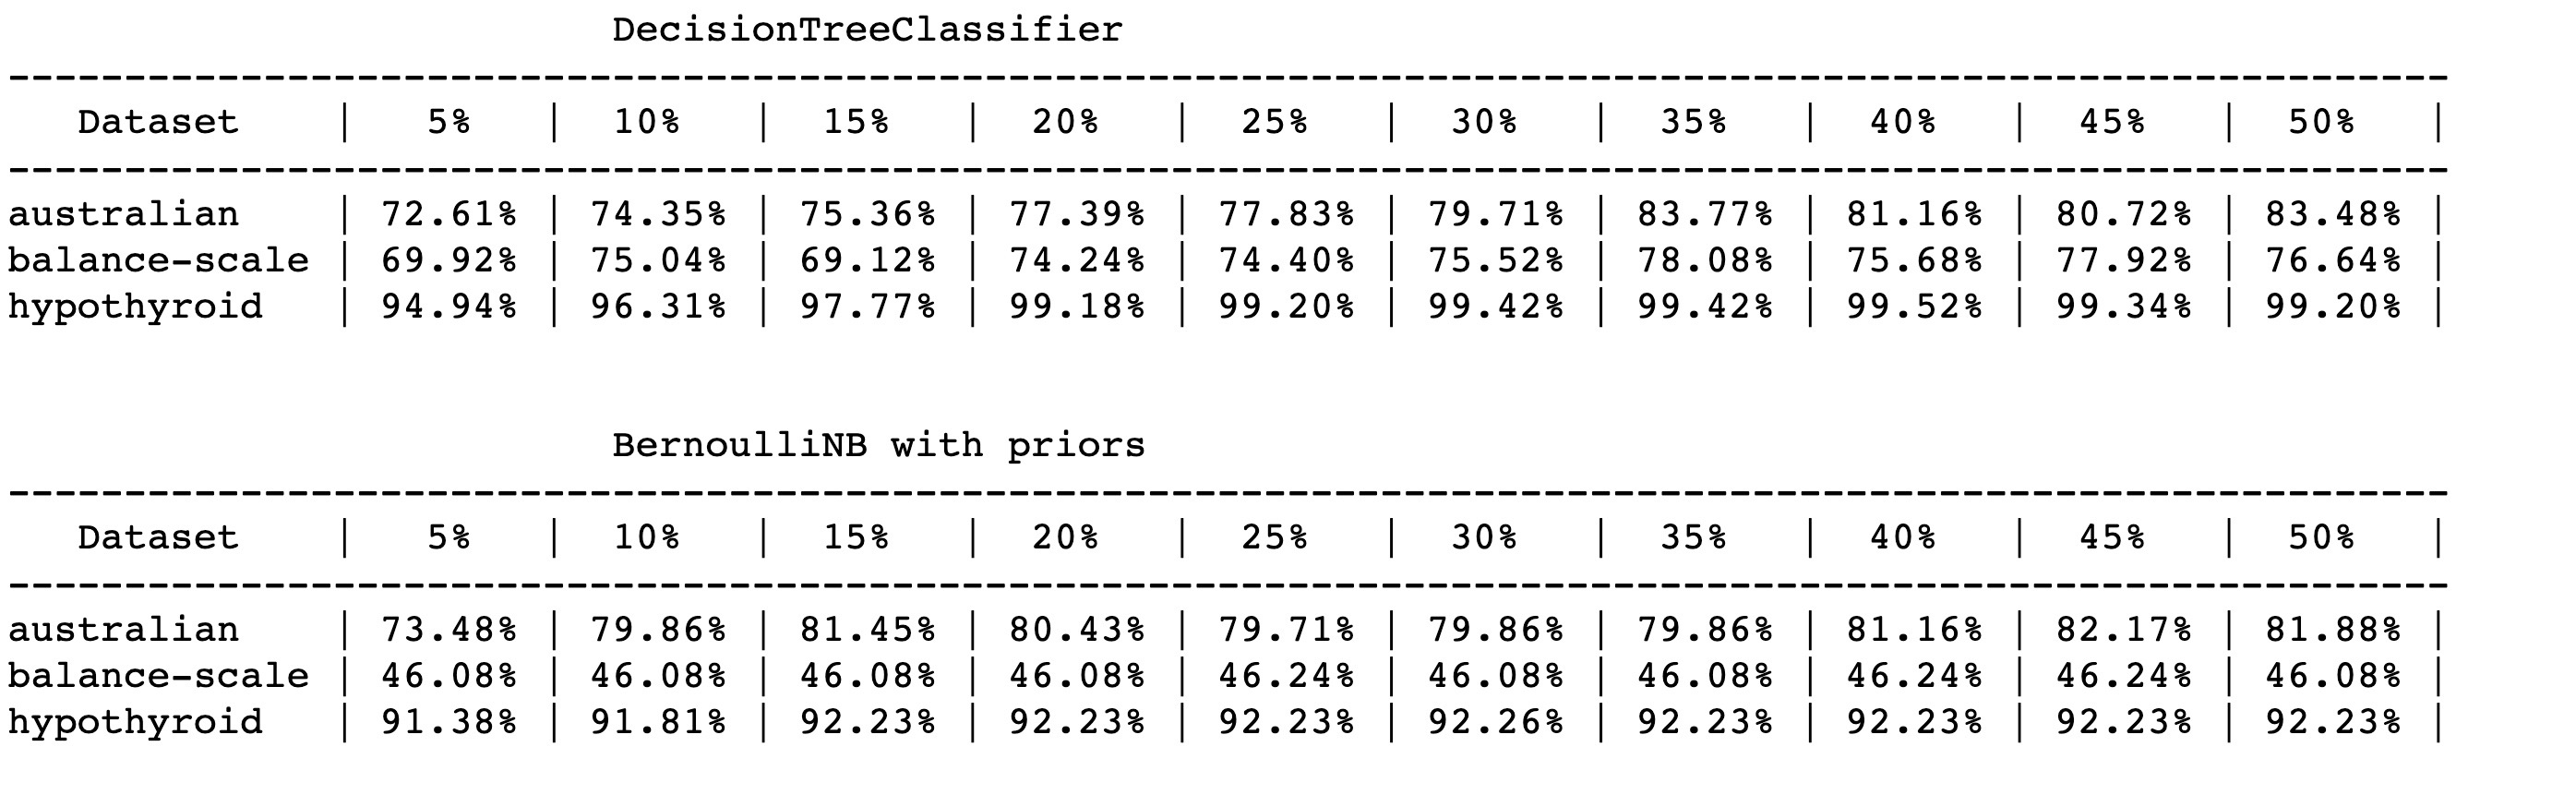
\includegraphics[scale=0.18]{result.jpeg}
    \subsection{Part B}\label{subsec:part-b}
    I think (3), (5) statements are true.
    \subsection{Part C}\label{subsec:part-c}
    I choose (1).
    \section{Q2}\label{sec:q2}
    \subsection{Part A}\label{subsec:part-a2}
    My accuracy score for the test dataset is 82.77\%. \\
    My accuracy score for the training dataset is 85.65\%.
    \subsection{Part B}\label{subsec:part-b2}
    The min\_samples\_leaf number of 5 to 7 give the optimal
    result, this can be observed by compare the auc score in
    the part c's plots, pick the maximum score with the lowest varience.
    \subsection{Part C}\label{subsec:part-c2}
    \begin{center}
        Plot For Test Dataset
    \end{center}
    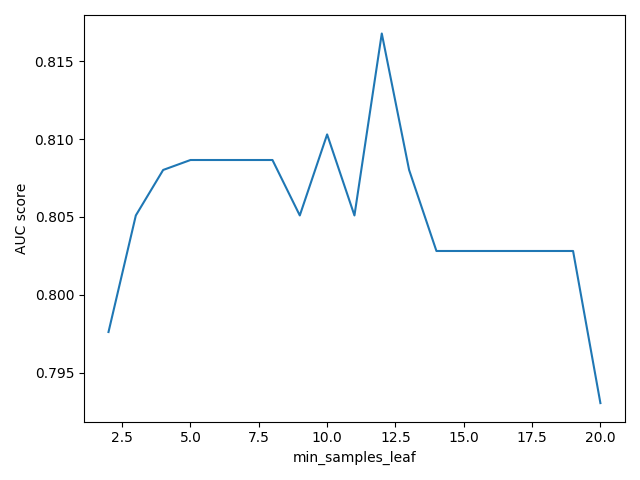
\includegraphics[scale=0.8]{../Plot/plot_test.png}
    \begin{center}
        Plot For Train Dataset
    \end{center}
    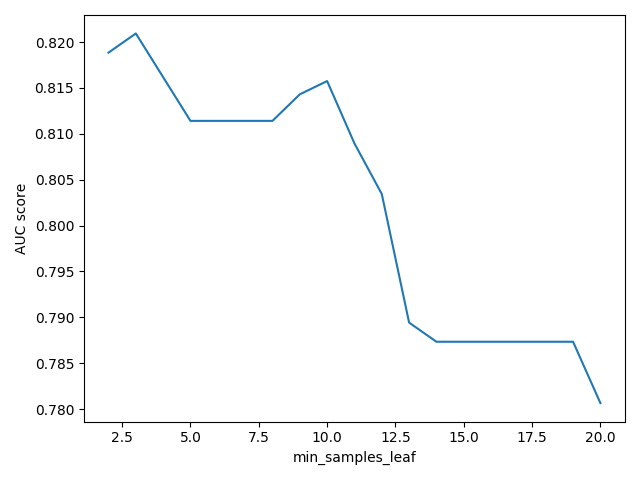
\includegraphics[scale=0.8]{../Plot/plot_train.png}
    \subsection{Part D}\label{subsec:part-d}
    We make the asumption that 'Sex' and 'Pclass' are independent feature. \\
    Thus, {\fontsize{9} P(S=true \lvert G=female,C=1)  = P(S= true \lvert G=female) *
    P(S=true \lvert C=1)} \\
    P(S=true \lvert G=female) = P(G=female) \cap P(S=true) / P(G=female) \\
    = 109 / 573 \\
    P(S=true \lvert C=1) = 136/216 \\
    P(S=true \lvert G=female,C=1) = 11.98\%.
    \subsection{My code}\label{subsec:my-code}
    \begin{lstlisting}
        import pandas as pd
        from sklearn.model_selection import train_test_split
        from sklearn import tree
        from sklearn.preprocessing import MinMaxScaler
        from sklearn.metrics import accuracy_score, roc_curve, auc


        # import numpy as np
        # import seaborn as sns
        # import graphviz
        # import matplotlib.pyplot as plt


        class TitanicSinkingModel:
        def __init__(self, filename):
        self.df = pd.read_csv(filename)
        self.df_normalized = None
        self.data_train = None
        self.data_test = None
        self.target_train = None
        self.target_test = None
        self.clf = None

        def preprocessing(self):
        # this can be done because the target value is either 0 or 1
        # thus apply the normalization have no effect on them
        scaler = MinMaxScaler()
        self.df_normalized = pd.DataFrame(scaler.fit_transform(self.df.values),
        columns=self.df.columns, index=self.df.index)
        self.split_dataframe()

        def split_dataframe(self):
        data = self.df_normalized[
        [col for col in self.df_normalized.columns if col != 'Survived']]
        target = self.df_normalized['Survived']
        # split the test and train data set
        self.data_train, self.data_test, self.target_train, self.target_test = train_test_split(data, target,
        test_size=0.3,
        shuffle=False)

        def fit_decision_tree(self):
        self.clf = tree.DecisionTreeClassifier()
        self.clf = self.clf.fit(self.data_train, self.target_train)

        # dot_data = tree.export_graphviz(clf, out_file=None)
        # graph = graphviz.Source(dot_data)
        # graph.format = 'jpg'
        # graph.render("decision_tree_plot_orignial")
        labels_test = self.clf.predict(self.data_test)
        acc = accuracy_score(labels_test, self.target_test)
        print("acc for test set is : " + str(acc))
        labels_test2 = self.clf.predict(self.data_train)
        acc2 = accuracy_score(labels_test2, self.target_train)
        print("acc for train set is : " + str(acc2))

        def find_optimal_decision_tree(self):
        # min_samples_leaf the minmum number of leaves a split
        # can happen according to the value of entropy
        auc_tain = {}
        auc_test = {}
        for i in range(2, 21):
        descion_tree = tree.DecisionTreeClassifier(min_samples_leaf=i)
        descion_tree.fit(self.data_train, self.target_train)
        false_positive_rate, true_positive_rate, thresholds = roc_curve(self.target_train, descion_tree.predict(self.data_train))
        auc_tain[i] = auc(false_positive_rate, true_positive_rate)
        false_positive_rate, true_positive_rate, thresholds = roc_curve(self.target_test, descion_tree.predict(self.data_test))
        auc_test[i] = auc(false_positive_rate, true_positive_rate)
        # fig = plt.figure()
        # d = {'min_samples_leaf': np.array(list(auc_tain)), 'AUC score': np.array(list(auc_tain.values()))}
        # pd_plot = pd.DataFrame(d)
        # sns.lineplot(x='min_samples_leaf', y='AUC score', data=pd_plot)
        # plt.show()
        # fig.savefig('plot_train.png')
        self.clf = tree.DecisionTreeClassifier(min_samples_leaf=6)
        self.clf.fit(self.data_train, self.target_train)
        # dot_data = tree.export_graphviz(self.clf, out_file=None)
        # graph = graphviz.Source(dot_data)
        # graph.format = 'jpg'
        # graph.render("decision_tree_plot_optimal")

        def part_D_calculation(self):
        print("female and survived: ")
        print(self.df.query('Sex == 1 & Survived ==1'))
        print("all female: ")
        print(self.df.query('Sex == 1'))
        print("first class and survived: ")
        print(self.df.query('Pclass == 1 & Survived ==1'))
        print("all first class: ")
        print(self.df.query('Pclass == 1'))


        def print_df_normalized(self):
        print(self.df_normalized.head().to_string())


        if __name__ == '__main__':
        titianic_sinking_model = TitanicSinkingModel("titanic.csv")
        titianic_sinking_model.preprocessing()
        # titianic_sinking_model.print_df_normalized()
        # print(titianic_sinking_model.data_train.to_string())
        titianic_sinking_model.fit_decision_tree()
        titianic_sinking_model.find_optimal_decision_tree()
        titianic_sinking_model.part_D_calculation()

    \end{lstlisting}

\end{document}